\documentclass{protokol}
\leftheader{Studium polarizace světla}
\centerheader{Praktikum III}
\rightheader{Tomáš Derner}

\begin{document}

  \section*{Úkol}

    \begin{enumerate}
      \item Stanovte ``směr snadného průchodu'' všech polarizátorů, které budete v úloze používat. Použijte odraz světla pod Brewsterovým úhlem na rozhraní vzduch-sklo (např. pomocí lampičky a zasklené fotografie připravené u úlohy).
      \item Ověřte platnost Malusova zákona.
      \item Proměřte jednu z následujících úloh:
      \begin{enumerate}
        \item závislost intenzity světla na úhlu pootočení polarizátoru, který je umístěn mezi dvěma dalšími polarizátory,
        \item stupeň polarizace světla, vzniklého lomem,
        \item kruhově a elipticky polarizované světlo (zpracujte do polárního grafu).
      \end{enumerate}
      \item Pozorujte, popište a vysvětlete dva z následujících efektů:
      \begin{enumerate}
        \item polarizaci odrazem pro různé úhly dopadu,
        \item indukovanou anizotropii,
        \item barevné efekty ve fázových destičkách,
        \item polarizaci rozptylem.
      \end{enumerate}
    \end{enumerate}

  \section*{Teorie}

    Elektromagnetické vlnění se dá popsat dvěma složkami elektrické intenzity kolmými na směr šíření vlny a na sebe navzájem. Tyto dvě složky mají na sobě nezávislé fázové posuny a vektor daný těmito složkami obecně opisuje elipsu \cite{teorie}, tedy toto vlnění má obecně eliptickou polarizaci.

    Polarizátory jsou optické prvky, které propouštějí jen světlo s určitou polarizací. Intenzitu propuštěného světla popisuje \textit{Malusův zákon}
    \begin{equation} \label{eq:malus}
      I = I_0 \cos^2 \psi,
    \end{equation}
    kde $I_0$ je intenzita dopadajícího světla a $\psi$ je úhel mezi vektorem intenzity elektrického pole a směrem snadného průchodu polarizátoru \cite{teorie}.

    Čtvrtvlnná destička umožňuje měnit excentricitu eliptické polarizace, tedy při natočení její rychlé osy o $\frac{\pi}{4}$ od roviny polarizace lineárně polarizovaného světla vystupuje po průchodu světlo kruhově polarizované. Je-li rychlá osa natočená vůči lineární polarizaci o násobky $\frac{\pi}{20}$, polarizace se nemění.

    Během měření byly využity aparatury popsané v \cite{pokyny}

  \section*{Výsledky}

    \subsection*{Úkol 1}

      Pomocí odrazu světla na skleněné destičce v okolí Brewsterova úhlu jsme určili směr snadného průchodu $\varphi$ tří polarizátorů vybavených úhlovými stupnicemi. Protože minima intenzity jsou okem snáze rozeznatelné, byly směry snadného průběhu spočteny přičtením/odečtením $\SI{90}{\degree}$ od naměřených minim. Protože měřené polarizátory byly držené ručně, což generuje určitou chybu v určení svislé polohy, a protože minimum intenzity světla nebylo možné určit přesně, byla těmto hodnotám přiřčena chyba $\SI{5}{\degree}$.

      $$ \varphi_1 = \SI{108}{\degree}, \SI{288}{\degree}, $$
      $$ \varphi_2 = \SI{154}{\degree}, \SI{335}{\degree}, $$
      $$ \varphi_3 = \SI{84}{\degree}, \SI{264}{\degree}. $$

    \subsection*{Úkol 2}

      Pro získání monochromatického světla byl do aparatury zařazen zelený monochromátor. 

      Postavením dvou polarizátorů do dráhy paprsku a postupným otáčením druhého s krokem $\SI{5}{\degree}$ jsme ověřili Malusův zákon \eqref{eq:malus}. Průběh závislosti intenzity na vzájemném otočení polarizátorů je zobrazen v grafu \ref{fig:u2}. Hodnoty naměřené intenzity nemají kvantitativní smysl, zajímavé jsou pouze relativní hodnoty vůči maximu.

      \begin{figure}[H]
        \centering
        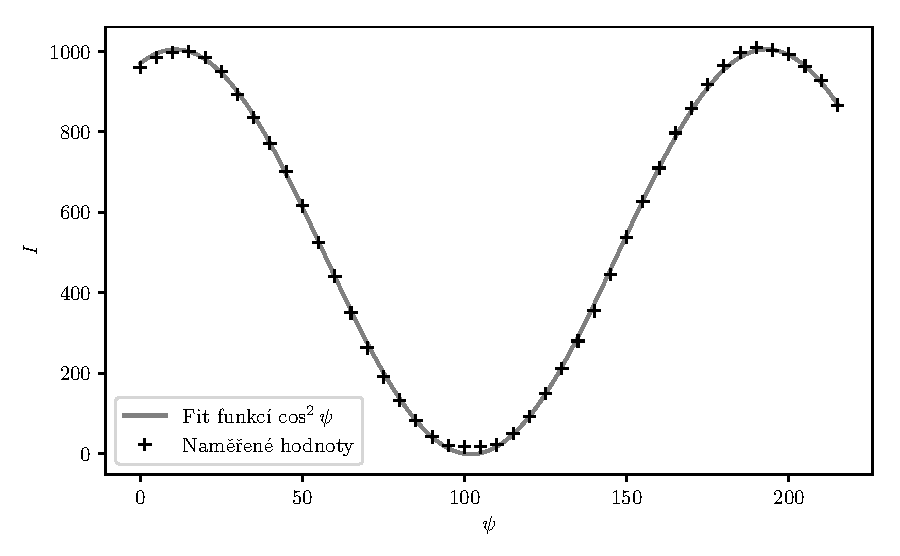
\includegraphics[]{u2}
        \caption{Závislost intenzity světla prošlého dvěma polarizátory na jejich relativním otočení}
        \label{fig:u2}
      \end{figure}

    \subsection*{Úkol 3}

      Byla měřena úloha \textit{c}: kruhově a elipticky polarizované světlo. 

      Mezi dva shodně natočené polarizátory byla umístěna čtvrtvlnná destička. Ta byla následně otáčena tak, aby intenzita světla dopadajícího na detektor byla maximální, tj. aby rychlá či pomalá osa destičky (v tomto experimentu jsou nerozlišitelné) měla stejný směr jako směr lineární polarizace světla. Následně byla destička otočena o $\SI{45}{\degree}$ pro první měření a poté vrácena a otočena o $\SI{15}{\degree}$.

      Měření probíhalo otáčením druhého polarizátoru krokem $\SI{5}{\degree}$ a zaznamenáváním prošlé intenzity. Výsledky měření jsou v grafu \ref{fig:u3}. 

      \begin{figure}[H]
        \centering
        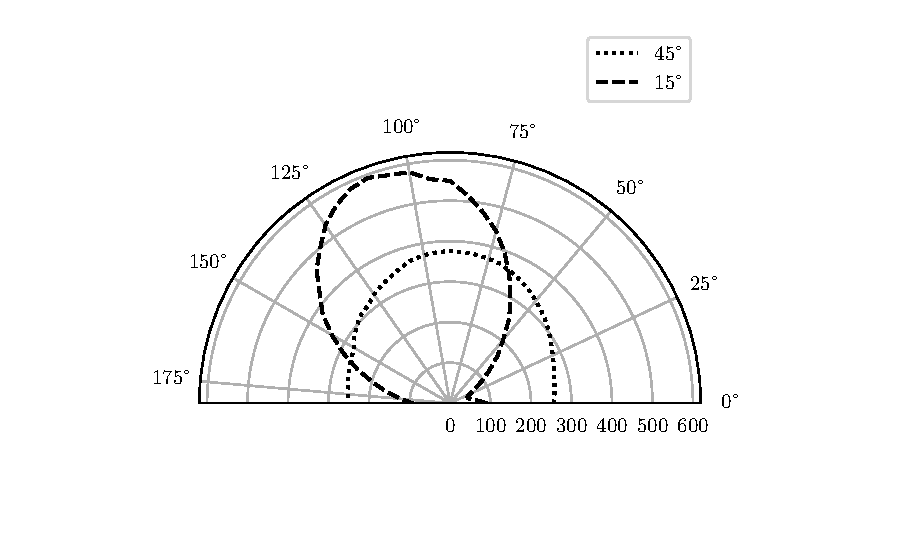
\includegraphics[]{u3}
        \caption{Závislost intenzity světla na úhlu natočení druhého polarizátoru}
        \label{fig:u3}
      \end{figure}

    \subsection*{Úkol 4}

      \subsubsection*{Indukovaná anizotropie}

        Mezi dva polarizátory byla umístěna plastová destička s rovnou dolní hranou a horní hranou vyříznutou do tvaru velmi rozevřeného V. Touto destičkou světlo procházelo homogenně, bez znatelných světlejších a tmavších míst.

        Když byla následně destička mechanicky namáhána, objevily se na ní světlá místa v oblasti působícího tlaku, kolem bodu zlomu tvaru horní hrany a ve střední části destičky po celé její délce. Tyto světlá místa odpovídají místům s velkým mechanickým napětím.

        Tento jev lze vysvětlit tím, že působením tlaku dochází v materiálu k dočasnému dvojlomu, tedy stejnému jevu, pomocí kterého fungují fázové destičky.
        V místech s dočasným dvojlomem dojde ke změně polarizace světla, což lze detekovat druhým polarizátorem.
 
      \subsubsection*{Barevné efekty ve fázových destičkách}

        Mezi dva polarizátory osvětlené bílým světlem byla vložena skleněná destička pokrytá na různých místech různým počtem vrstev průhledné lepicí pásky. Tato místa byla v závislosti na tloušťce vrstvy pásky různě zbarvena.

        Toto je opět způsobeno dvojlomem a páska funguje jako fázová destička. Protože působení fázové destičky je závislé na vlnové délce světla, jen některé barvy světla budou páskou polarizovány ve směru snadného průchodu druhého polarizátoru.

        Efekt dvojlomu je v pásce pravděpodobně způsoben při určitém kroku výroby, kdy je páska natahována v jednom směru.

  \section*{Diskuse}

    Z grafu \ref{fig:u2} je zřejmé, že měřicí přístroj nebyl schopen spolehlivě zachytit velmi malé intenzity světla a minimum naměřeného průběhu je proto mírně zdeformované. Mimo to bylo však ověření Malusova zákona poměrně přesné. Určitá chyba v této části měření mohla vzniknout tím, že nebylo příliš dbáno na otáčení polarizátoru přesně o pět stupňů v každém kroku, naměřené hodnoty tak mají každá chybu asi dva stupně. Tyto chyby se však v lineární regresi více méně kompenzují.

    Ačkoli byla při měření úkolu 3 destička otočena co nejpřesněji o $\SI{45}{\degree}$ a jak poloha os destičky vůči polarizátorům, tak i toto otočení bylo několikrát kontrolováno a opravováno, nebylo možné vytvořit uspokojivě kruhovou polarizaci. Tato zvláštnost se pak pravděpodobně projevila i při druhém měření, kdy nevyšla v polárním grafu elipsa, jak předpovídá teorie.

  \section*{Závěr}
      
    Byly určeny směry snadného průchodu polarizátorů
    $$ \varphi_1 = \SI{108}{\degree}, \SI{288}{\degree}, $$
    $$ \varphi_2 = \SI{154}{\degree}, \SI{335}{\degree}, $$
    $$ \varphi_3 = \SI{84}{\degree}, \SI{264}{\degree}. $$

    Byl uspokojivě ověřen Malusův zákon.

    Byla změřena závislost intenzity světla prošlého čtvrtvlnnou destičkou mezi dvěma polarizátory na úhlu natočení druhého polarizátoru.

    Byly popsány jevy indukovaná anizotropie a barevné efekty ve fázových destičkách. Obojí je způsobeno dvojlomem.

  \begin{thebibliography}{}
 
    \bibitem{teorie}
    Studijní text ``Polarizace světla'', dostupné z\\ \url{http://physics.mff.cuni.cz/vyuka/zfp/_media/zadani/texty/txt_323.pdf}, 28.\,3.\,2018

    \bibitem{pokyny}
    Pokyny k měření ``Studium polarizace světla'', dostupné z\\ \url{http://physics.mff.cuni.cz/vyuka/zfp/_media/zadani/pokyny/mereni_323.pdf}, 28.\,3.\,2018
   
  \end{thebibliography}

\end{document}